\documentclass[letterpaper, 12]{article}

%% Language and font encodings
\usepackage[english]{babel}
\usepackage[utf8x]{inputenc}
\usepackage[T1]{fontenc}

%% Sets page size and margins
\usepackage[letterpaper,top=2.5cm,bottom=2cm,left=2cm,right=2cm,marginparwidth=1.75cm]{geometry}

%% Useful packages
\usepackage{amsmath}
\usepackage{amssymb}
\usepackage{amsfonts}
\usepackage{graphicx}
\usepackage{physics}
\usepackage{bbold}
\usepackage[colorinlistoftodos]{todonotes}
\usepackage[colorlinks=true, allcolors=blue]{hyperref}
\usepackage{listings}
\usepackage{multicol}
\usepackage{float}
\usepackage{enumitem}

\usepackage{bm}
\date{\today}

\title{CSC411 Assignment 3}
\author{Yue Guo}
\begin{document}
\maketitle

%%%%%%%%%%%Q1 	20 NEWS GROUP  %%%%%%%%%%%%%%
\section{20 News Group}
\subsection{Top 3 Algorithms}
\subsubsection{Neural Network}
\begin{enumerate}

    \item Hypterparameter
	
	In the code nn\_news, I have tried a single layer neural network vs multi-layered neural network. It turns out that the single neural network is the fastest and also most accurate.

	\item Train/test loss
	\begin{itemize}
     \item  Train accuracy
     \item Test accuracy
        \end{itemize}
      \item My expectations
  
\end{enumerate}

\subsubsection{Random forest}
\begin{enumerate}

    \item Hypterparameter
	
	In the code nn\_news, I have tried a single layer neural network vs multi-layered neural network. It turns out that the single neural network is the fastest and also most accurate.

	\item Train/test loss
	\begin{itemize}
     \item  Train accuracy
     \item Test accuracy
        \end{itemize}
      \item My expectations
  
\end{enumerate}

\subsubsection{SVM - Best Classifier}
\begin{enumerate}

    \item Hypterparameter
	
	In the code nn\_news, I have tried a single layer neural network vs multi-layered neural network. It turns out that the single neural network is the fastest and also most accurate.

	\item Train/test loss
	\begin{itemize}
     \item  Train accuracy  0.972511932119
     \item Test accuracy 0.691980881572
        \end{itemize}
      \item My expectations
  
\end{enumerate}

\subsubsection{Bernoulli Baseline}
\begin{enumerate}
	\item Train/test loss
	\begin{itemize}
     \item  Train accuracy  0.598727240587
     \item Test accuracy 0.457912904939
        \end{itemize}
\end{enumerate}





%%%%%%%%%%%Q2 SVM %%%%%%%%%%%%%%
\section{SVM}
\begin{figure}[H]
\centering
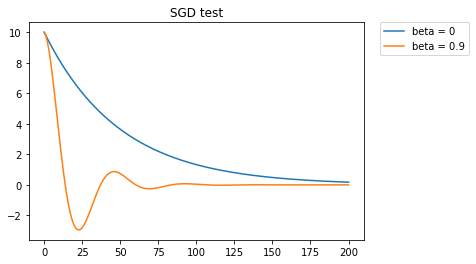
\includegraphics[width=0.5\textwidth]{q2part1plot.png}
\caption{\label{}Plot of test SVM}
\end{figure}


%%%%%%%%%%%Q3%%%%%%%%%%%%%%
\section{Kernels}
%%%%%%%%%% q 3.1%%%%%%%%%%%%%%
\subsection{Positive semidefinite and quadratic form}
Assume K is symmetric, we can decompose K into $U \Lambda U^T$
\begin{equation*}
\begin{split}
x^T K x &= x^T (U \Lambda U^T) x = (x^T U) \Lambda (U^T x)\\
\end{split}
\end{equation*}

$\Lambda$ has the eigenvalues $\lambda_{i}$, and if $K$ is positive, and all $\lambda_{i}$ > 0,

\begin{equation*}
\begin{split}
x^T K x &= \Sigma_{i =1}^{d} \lambda_{i} ([x^T U_{i}])^2 >= 0\\
\end{split}
\end{equation*}

Then $x^T K x >= 0$ for all $x$ in $ \mathbb{R}^{d}$

%%%%%%%%%Q 3.2 %%%%%%%%%%%%%%
\subsection{Kernel properties}
%%%%%%%% Q 3.2 q2%%%%%%%%%%%%%
\subsubsection{$\alpha$}
Define mapping $\phi (x) = \sqrt{\alpha}$, $\alpha > 0$, and the kernel $\langle \phi(x), \phi(y) \rangle = \alpha$.
The resulting matrix K has item $K_{ij} = \alpha $, the matrix K has equal number of row and columns, and each element is $\alpha$. Since $\alpha$ > 0, and all elements are equal, K is positive semidefinite
 
 %%%%%%%Q 3.2 q3 %%%%%%%%%%%%%%
\subsubsection{$f(x), f(y)$}
$K_{ij} = \langle \phi (x),  \phi (y) \rangle$, \\
define $\phi(x) = f(x), \forall f: \mathbb{R}^{d} \rightarrow \mathbb{R}$\\
define $\phi(y) = f(y), \forall f: \mathbb{R}^{d} \rightarrow \mathbb{R}$\\
Since f(x) and f(y) produce a scalar,  $\langle \phi (x),  \phi (y) \rangle = f(x) \cdot f(y)$

%%%%%%%%Q3.2 part 3%%%%%%%%%%%
\subsubsection{k1 and k2}
If the gram matrix, $K_{1}$ of kernel k1 and gram matrix, $K_{2}$ of kernel k2 are positive semidefinite, by scaling them and adding each element, the new gram matrix of $a \cdot k_{1}(x, y) + b \cdot k_{2}(x, y)$, call it $K$, each element of K is positive since a ,b > 0.\\
$K$ is also symmetric because $K_{1}$ and $K_{2}$ are symmetric with the same dimension, and element wise addition and linear combination preserve the symmetric property.\\

%%%%%%%%Q3.2 part 4%%%%%%%%%%%
\subsubsection{$k(x, y) = \frac{k_{1}(x ,y) }{\sqrt{k_{1}(x, x)} \sqrt{k_{1}(y, y)} }$}
Let $\phi_{1}$ be the mapping defined by $k_{1}$\\
We define a new mapping, $\phi$ for $k(x ,y)$\\
We let $\phi(x) = \frac{\phi_{1} (x)}{\norm{\phi_{1}(x)}}$\\
\begin{equation*}
\begin{split}
k(x, y) &= \langle \phi (x), \phi (y) \rangle \\
&= \frac{\phi_{1}(x)}{\norm{\phi_{1}(x)}} \cdot  \frac{\phi_{1}(y)}{\norm{\phi_{1}(y)}}\\
&= \frac{\phi_{1}(x)}{\sqrt{\phi_{1}(x) \cdot \phi_{1}(x)}} \cdot \frac{\phi_{1}(y)}{\sqrt{\phi_{1}(y) \cdot \phi_{1}(y)}}\\
&= \frac{\phi_{1}(x)}{( \sqrt{\phi_{1}(x)} \cdot \sqrt{ \phi_{1}(y)}  )}  \cdot \frac{\phi_{1}(y)}{( \sqrt{\phi_{1}(x)} \cdot \sqrt{ \phi_{1}(y)}  )} \\
&= \frac{\phi_{1}(x)}{ \sqrt{\phi_{1}(x) \cdot  \phi_{1}(y) }}  \cdot  \frac{\phi_{1}(x)}{ \sqrt{\phi_{1}(x) \cdot  \phi_{1}(y) }}\\
 k(x, y) &= \frac{k_{1}(x ,y) }{\sqrt{k_{1}(x, x)} \sqrt{k_{1}(y, y)} }
\end{split}
\end{equation*}
Therefore, there is a new mapping $\phi(x)$ that supports $k(x, y)$ and it is a kernel because $\phi(x)$
is the product of two kernel mappings

\end{document}